\documentclass[12pt, a4paper, twoside]{pancake-book}

% NOTE *** preamble ***
\setlength{\headheight}{14.49998pt} % make latex stop complaining!

% simpler commands
\renewcommand*{\bf}[1]{\textbf{#1}}
\renewcommand*{\it}[1]{\textit{#1}}
\renewcommand*{\tt}[1]{\texttt{#1}}

% math macros
\newcommand*{\f}[2]{\frac{#1}{#2}}
\newcommand*{\slf}[2]{\slashfrac[auto]{#1}{#2}}
\newcommand*{\reals}{\mathbb{R}}
\newcommand*{\ints}{\mathbb{Z}}
\newcommand*{\rationals}{\mathbb{Q}}
\newcommand*{\naturals}{\mathbb{N}}

% define colours used throughout the document
\definecolor{accent}{HTML}{EF476F}
\definecolor{razz}{HTML}{DB3069} % pink -- all of these colours are very vibrant
\definecolor{cobalt}{HTML}{1446A0} % blue
\definecolor{naples}{HTML}{F5D547} % yellow

% wrap figures
\usepackage{wrapfig}

% maths
\usepackage{mathtools, amsthm, amssymb, amsmath}
\usepackage{derivative}

% expandable brackets
\usepackage{physics2}
\usephysicsmodule[tightbraces=true]{ab}

% chemistry
\usepackage{chemformula, chemmacros}
\NewChemCompoundProperty{l}{\textit{l}}

% si units
\usepackage{siunitx}
\sisetup{
	mode=match,
	propagate-math-font=true,
	reset-math-version=false,
	reset-text-family=false,
	reset-text-series=false,
	reset-text-shape=false,
	text-family-to-math=true,
	text-series-to-math=true,
}
\DeclareSIUnit{\conc}{\mol\per\deci\meter\cubed}
\DeclareSIUnit{\concrate}{\conc\per\second}
\DeclareSIUnit{\year}{year}
\DeclareSIUnit{\electron}{electron}
\DeclareSIUnit{\atom}{atom}
\DeclareSIUnit{\epera}{\electron\per\atom}
\DeclareSIUnit{\atm}{atm}

% fonts: unfortunately i've to use `pdflatex' here
\usepackage{fontspec}
\usepackage{unicode-math}
\setmainfont{STIX Two Text}[Ligatures=TeX]
\setmathfont{STIX Two Math}[Ligatures=TeX]
\setsansfont{TeX Gyre Heros}[Ligatures=TeX]
\setmonofont{JetBrains Mono}[Ligatures=TeX]

% use sans font for headers and footers
\fancyhf{}
\fancyfoot[LE,RO]{\small\sffamily\thepage}
\fancyhead[LE]{\small\sffamily\scshape\nouppercase\leftmark}
\fancyhead[RO]{\small\sffamily\nouppercase\rightmark}

% everything about graphs and figures
\usepackage{pgfplots, pgfplotstable}
\pgfplotstableset{col sep=comma}
\usetikzlibrary{
	positioning,
	calc,
	shapes,
	backgrounds,
	fit,
	decorations,
	arrows,
	arrows.spaced,
	intersections,
	3d,
	tikzmark,
}
\usepgfplotslibrary{
	colorbrewer,
	units,
	dateplot,
	fillbetween,
	groupplots,
}
\pgfplotscreateplotcyclelist{mod RdYlBu3}{
	{accent},
	{cobalt},
	{naples},
}
\pgfplotscreateplotcyclelist{mod mark list}{
	every mark/.append style={solid,fill=\pgfplotsmarklistfill}\\
	every mark/.append style={solid,fill=\pgfplotsmarklistfill},mark=*\\
	every mark/.append style={solid,fill=\pgfplotsmarklistfill},mark=square*\\
	every mark/.append style={solid,fill=\pgfplotsmarklistfill},mark=triangle*\\
	every mark/.append style={solid},mark=star\\
	every mark/.append style={solid,fill=\pgfplotsmarklistfill},mark=diamond*\\
	every mark/.append style={solid,fill=\pgfplotsmarklistfill!40},mark=otimes*\\
	every mark/.append style={solid},mark=|\\
	every mark/.append style={solid,fill=\pgfplotsmarklistfill},mark=pentagon*\\
}
\pgfplotsset{
	width=8cm,
	compat=1.16,
	clip mode=individual,
	label style={font=\small},
	tick label style={
		font=\small,
		/pgf/number format/1000 sep={\,}
		/pgf/number format/precision=3,
		/pgf/number format/fixed,
		/pgf/number format/fixed zerofill,
	},
	legend style={
		at={(0.5, 1.05)},
		anchor=south,
		legend columns=-1,
		font=\footnotesize,
		draw=none,
		fill=none,
	},
	colormap/viridis,
	unit code/.code 2 args={\unit{#1#2}},
	unit markings={slash space},
	every axis plot post/.append style={
		align=center,
		ultra thick,
		axis lines=left,
		axis x line=bottom,
		axis y line=left,
		axis line style={semithick},
		enlargelimits=0.05,
	},%
	cycle multi list={
		mod mark list\nextlist
		linestyles*\nextlist
		mod RdYlBu3
	},
}

% fun highlights
\usepackage{tcolorbox}
\tcbuselibrary{breakable, skins}
\newtcbox{\hil}[1][accent]{
	on line,
	arc=0pt,
	outer arc=0pt,
	colback=#1!25!white,colframe=#1,
	boxsep=0pt,left=1pt,right=1pt,top=2pt,bottom=2pt,
	boxrule=0pt,bottomrule=1pt,toprule=1pt,
	breakable,enhanced jigsaw,
}

% coloured links
\usepackage{hyperref}
\hypersetup{
	hidelinks,
	colorlinks=true,
	breaklinks=true,
	urlcolor=razz,
	bookmarksopen=false,
	pdftitle={SJChO},
	pdfauthor={Darren Yap},
	linkcolor=cobalt,
}

% make sure align*, aligned environments can stretch across pages
\allowdisplaybreaks

% better chapter headings
\titleformat{\subsubsection}[hang]{
	\sffamily\itshape\normalsize\color{accent}
}{\thesubsubsection}{.5em}{}

% finally we get to it
\title{SJChO: Homework}
\author{Darren \color{accent} Yap}
\date{2024}

\begin{document}
\maketitle
\tableofcontents

\setcounter{chapter}{5}

% all our chapters, in order
\chapter{Reaction Kinetics}
\section{Homework: Reaction Kinetics}
\subsection{Redox}
\subsubsection{Problem}
Hydrogen peroxide reacts with acidified iodide ions, liberating iodine.
In investigations of this reaction, the following results were
obtained (Table~\ref{tab:h2o2}).
\begin{table}[htpb]
	\centering
	\footnotesize
	\begin{tabular}{l r r r r}
		\toprule
		Experiment & \ch{[H2O2]}/\unit{\milli\conc} & \ch{[I^-]}/\unit{\milli\conc} & \ch{[H^{+}]}/\unit{\milli\conc} & Initial rate/\unit{\milli\concrate} \\
		\midrule
		1          & \num{10.0}                     & \num{9.0}                     & \num{10.0}                      & \num{2.30e-3}                       \\
		2          & \num{34.0}                     & \num{9.0}                     & \num{10.0}                      & \num{7.82e-3}                       \\
		3          & \num{34.0}                     & \num{13.5}                    & \num{10.0}                      & \num{1.75e-2}                       \\
		4          & \num{34.0}                     & \num{9.0}                     & \num{24.0}                      & \num{7.82e-3}                       \\
		\bottomrule
	\end{tabular}
	\caption{Results for reaction between \ch{H2O2} and \ch{I-}}
	\label{tab:h2o2}
\end{table}

\begin{enumerate}
	\item Determine the rate equation of this reaction.
	\item Calculate the rate constant and state its units.
\end{enumerate}

\subsubsection{Solution}
Since the initial rate increases linearly with \ch{[H2O2]}, the reaction
is first-order w.r.t. \ch{[H2O2]}. The reaction is second-order w.r.t. \ch{[I^-]}
and zeroth-order w.r.t. \ch{[H^{+}]}. Therefore, the rate equation is (Equation~\ref{eq:rateeq-h2o2})

\begin{equation}
	\color{accent}
	v = k \ch{[H2O2]} {\ch{[I^-]}}^2
	\label{eq:rateeq-h2o2}
\end{equation}

We can substitute the values from Experiment 1 into Equation~\ref{eq:rateeq-h2o2}.
\begin{align*}
	\num{2.30e-3} & = k \left(10.0\right) \ab(9.0)^2                         \\
	k             & = \f{\num{2.30e-3}}{\num{810.0}}                         \\
	              & = \color{accent} \qty{2.84e-6}{mmol^{-2}.dm^{-6}.s^{-1}} \\
\end{align*}

\subsection{Decomposition Graphs}
\subsubsection{Problem}
The decomposition of \ch{N2O4} is found to be \textbf{first-order}
with respect to \ch{[N2O4]} (Figure~\ref{fig:graphs}).
Which of the following graphs confirms the above finding? For the graphs that are incorrect, copy the axes
and sketch the correct shape of the graph.
\begin{figure}
	\centering
	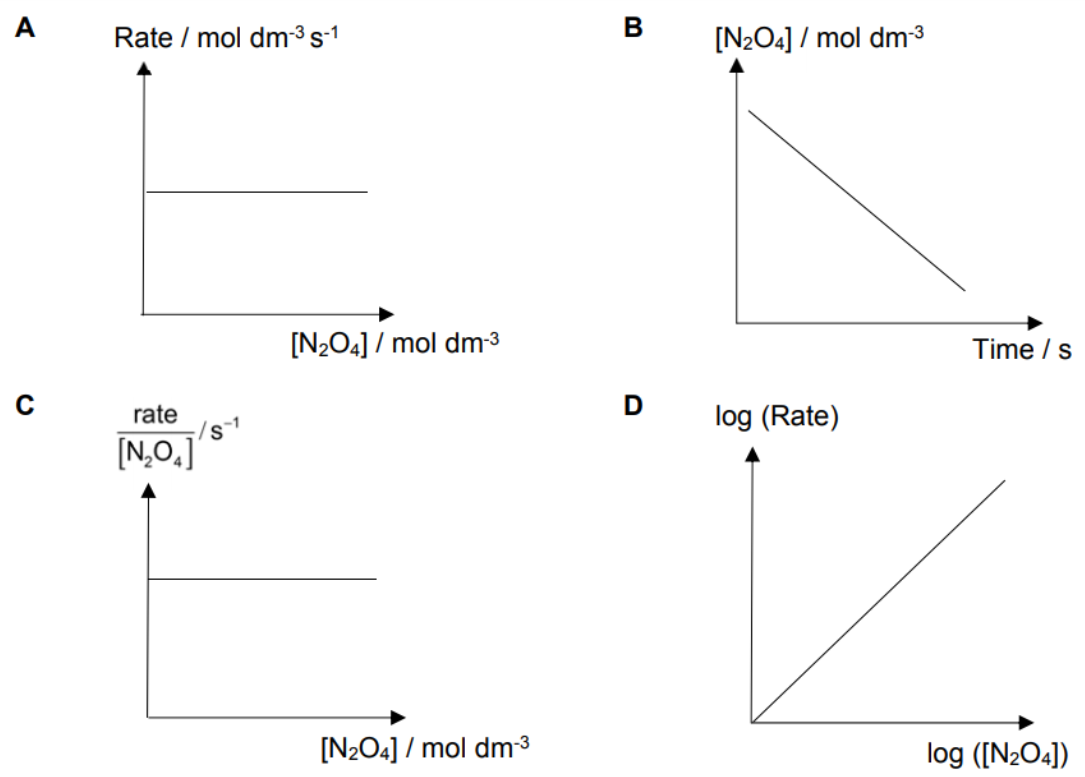
\includegraphics[width=0.90\linewidth]{assets/06_n2o4.png}
	\caption{Various graphs of the decomposition of \ch{N2O4}}
	\label{fig:graphs}
\end{figure}

\begin{itemize}
	\item Graph \textbf{A} is {\color{accent} incorrect}. It illustrates a zeroth-order decomposition instead of a first-order one. The correct shape is:
	      \begin{center}
		      \begin{tikzpicture}
			      \begin{axis}[
					      ticks=none,
					      xmin=0,ymin=0,xmax=3,ymax=3,
					      xlabel={\(\slf{\ch{[N2O4]}}{\unit{\conc}}\)},
					      ylabel={\(\slf{v}{\unit{\concrate}}\)},
				      ]
				      \addplot+[dotted]{1.5};
				      \addplot{x};
			      \end{axis}
		      \end{tikzpicture}
	      \end{center}
	\item Graph \textbf{B} is {\color{accent} correct}. Since \(v = -\odv{\ch{[N2O4]}}/{t}\)
	      and \ch{N2O4} undergoes first-order decomposition, \ch{[N2O4]} should decrease
	      linearly too.
	\item Graph \textbf{C} is {\color{accent} correct}. Since \(v = k\ch{[N2O4]}\),
	      \(k = \slf{v}{\ch{[N2O4]}}\), a constant.
	\item Graph \textbf{D} is {\color{accent} incorrect}. The graph of \(v\) against
	      \ch{[N2O4]} is linear, so the graph of \(\log v\) against \(\log \ch{[N2O4]}\)
	      should follow a logarithmic curve:
	      \begin{center}
		      \begin{tikzpicture}
			      \begin{axis}[
					      ticks=none,
					      xmin=0,ymin=-1,xmax=5,ymax=5,
					      xlabel={\(\log \ch{[N2O4]}\)},
					      ylabel={\(\log v\)},
					      ticks=none,
				      ]
				      \addplot+[dotted]{x};
				      \addplot{ln x};
			      \end{axis}
		      \end{tikzpicture}
	      \end{center}
\end{itemize}

\subsection{Carbon Dating}
\subsubsection{Problem}
Carbon-14 dating is a technique used to estimate the age of organic material. A living organism constantly exchanges carbon with the environment, thus the amount
of radioactive carbon-14 in the organism stays constant at around 1 part per trillion.
When the organism dies, the amount of carbon-14 starts to decrease due to radioactive decay, following first-order kinetics with a decay constant of \qty{1.21e-4}{\per\year}.

\begin{enumerate}
	\item The human body comprises roughly \qty{16}{\kilo\gram} of carbon. Estimate the number of carbon-14 atoms present in a living human.
	\item When one carbon-14 atom decays, one electron is emitted. Calculate the rate of emission of electrons from a living human, giving your answer in electrons per second.
	\item The rate of electron emission from an ancient Egyptian mummy was detected to be \qty{2000}{electron.s^{-1}}. Estimate the age of the mummy.
\end{enumerate}

\begin{align*}
	\text{Total mass of all \ch{^{14}C} atoms} & = \qty{16e-12}{\kilogram}                            \\
	                                           & = \qty{1.6e-11}{\kilogram}                           \\
	                                           & = \qty{1.6e-8}{\gram}                                \\
	\\
	\eta_{\ch{^{14}C}}                         & = \qty{1.6e-8}{\gram}/\qty{14}{\gram\per\mol}        \\
	                                           & = \qty{1.14e-9}{\mol}                                \\
	\\
	n_{\ch{^{14}C}}                            & = \qty{1.14e-9}{\mol} \times \qty{6.02e23}{\per\mol} \\
	                                           & = \color{accent} \num{6.88e14}
\end{align*}


\begin{align*}
	\text{Decay rate} & = \ab(\num{6.88e14})\ab(\qty{1}{\epera})\ab(\qty{1.21e-4}{\per\year})      \\
	                  & = \ab(\num{6.88e14})\ab(\qty{1}{\epera})\ab(\qty{3.8369e-12}{\per\second}) \\
	                  & = \color{accent} \qty{2.64e3}{electron.s^{-1}}
\end{align*}


Let \(t\) be the age of the mummy. \(n_t\) is the number of
\ch{^{14}C} atoms after time \(t\), and \(n_0\) is that in
the mummy while still alive.
\begin{align*}
	n_t                                              & = \frac{\ab(\qty{2e3}{electron.s^{-1}})\ab(\qty{3.154e7}{\second\per\year})}{\qty{1.21e-4}{\per\year}} \\
	                                                 & = \qty{5.213e14}{atom}                                                                                 \\
	                                                 & = \qty{5.213e14}{electron}                                                                             \\
	\\
	t_{\slf{1}{2}}                                   & = \frac{\ln 2}{\lambda}                                                                                \\
	                                                 & = \frac{\ln 2}{\qty{1.21e-4}{\per\year}}                                                               \\
	                                                 & = \qty{5728.49}{\year}                                                                                 \\
	\\
	\because \; n_t                                  & = n_0 \ab(\frac{1}{2})^{\slf{t}{t_{\slf{1}{2}}}}                                                       \\
	\therefore \; \qty{5.213e14}{electron}           & = \ab(\qty{6.88e14}{electron})\ab(\frac{1}{2})^{\slf{t}{\qty{5728.49}{\year}}}                         \\
	\ab(\frac{1}{2})^{\slf{t}{\qty{5728.49}{\year}}} & = \num{0.7577}                                                                                         \\
	t                                                & = \num{5728.49} \log_{\slf{1}{2}}{0.7577}                                                              \\
	                                                 & = \color{accent} \qty{2293}{\year}
\end{align*}

\chapter{Equilibrium}

\section{Rod and spring}
\begin{problem}
  In \cref{fig:rodspring}, a uniform rod of mass \qty{8.0}{\kg} and
  length \qty{0.50}{\metre}
  is pivoted about point \(P\). It is held in position by a spring of
  original length \qty{0.20}{\metre},
  spring constant \qty{5.0e2}{\newton\per\metre}, and negligible mass.
  Determine the length \(x\).
\end{problem}
\begin{wrapfigure}{i}{0.5\textwidth}
  \centering
  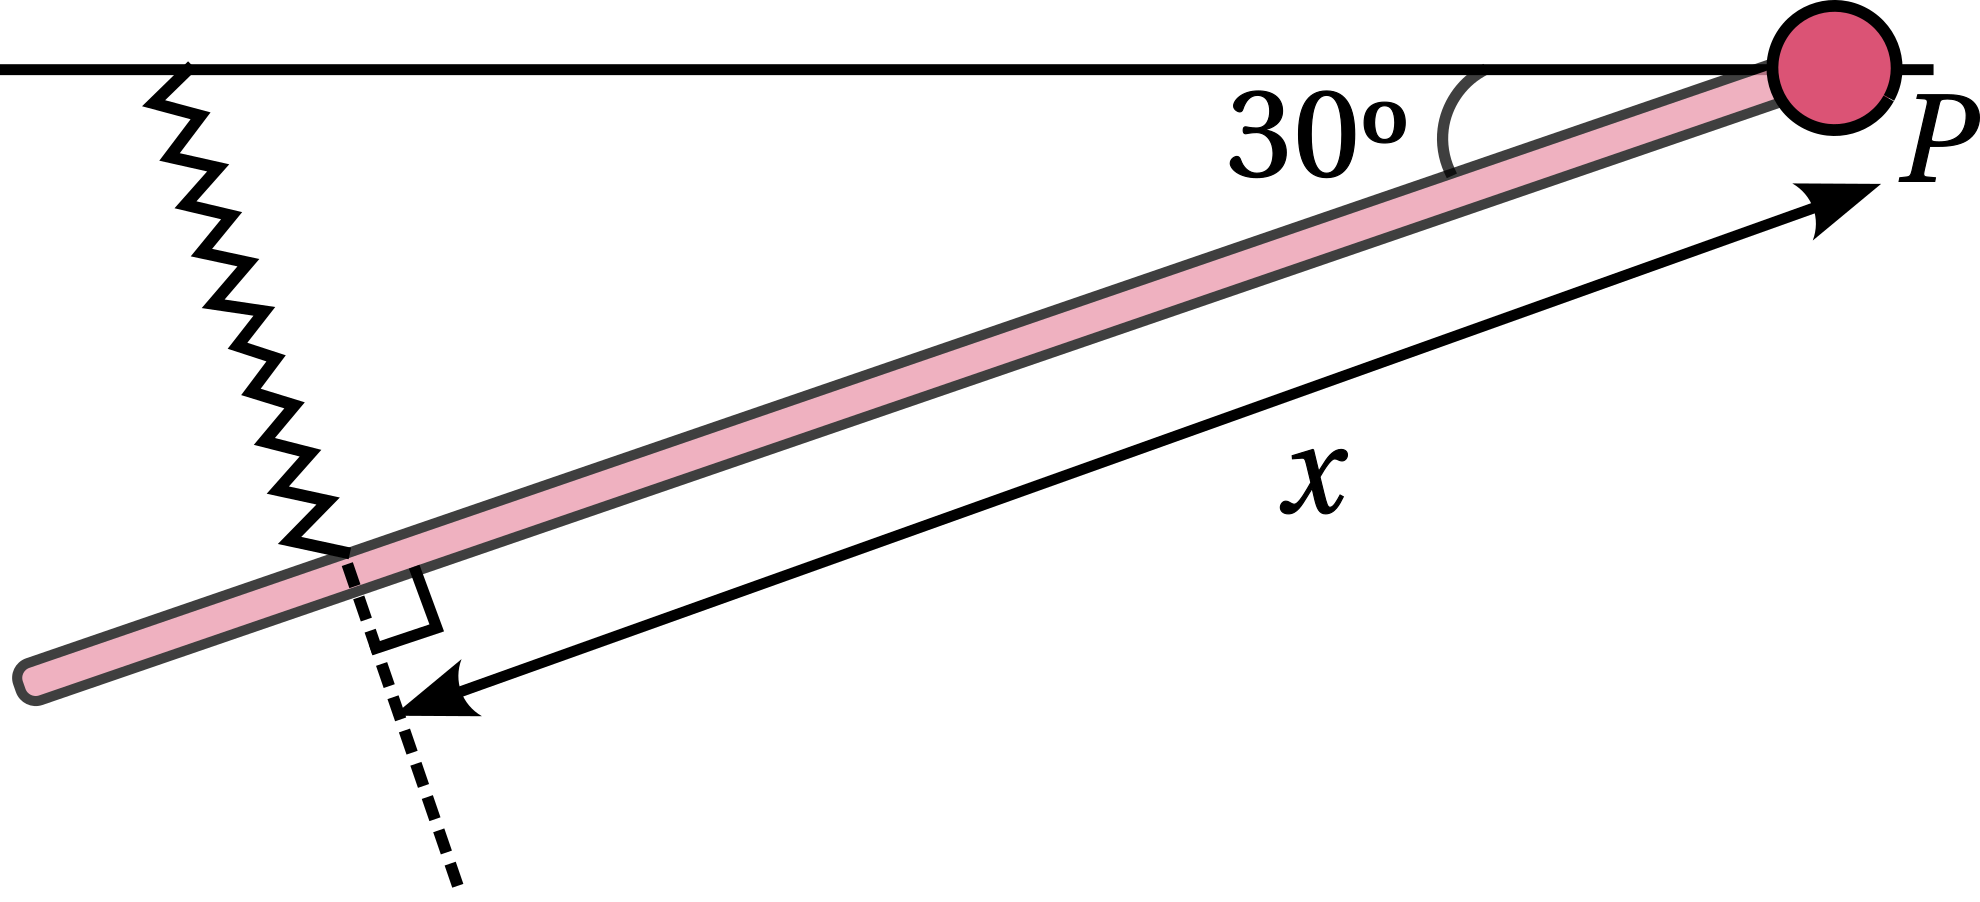
\includegraphics[width=0.48\textwidth]{assets/rodspring.png}
  \caption{Rod and spring}
  \label{fig:rodspring}
\end{wrapfigure}
We define our variables. Let
\begin{itemize}
  \item \(e\) be the extension of the spring, \(l_s\) be its original
    length, and \({l_s}'\) be its stretched length;
  \item \(k_s\) be the spring constant;
  \item \(m\) be the mass of the rod, and \(l_r\) be its length; and
  \item \(\theta\) be the angle the rod makes with the wall.
\end{itemize}

The stretched spring, the rod (up to a distance \(x\) away from the
pivot) and the wall
form a right-angled triangle. The stretched length \({l_s}' = x \tan \theta\).
Therefore, the extension of the spring \(e = {l_s}'-l_s = x\tan\theta - l_s\).

The elastic force generated by the spring \(F_s\) is determined to be
\begin{equation}
  \mv{F}_s = k_se = k_s\ab(x\tan\theta-l_s)
  \label{eq:elasticforce}
\end{equation}

Also acting on the body of the rod, the weight of the rod \(\mv{W} = mg\). Since
the rod's weight does not act perpendicularly to the rod in this instance, we
can resolve its weight into its vertical component. Furthermore, since the rod
is \term{uniform}, its weight acts in the geometrical centre of its
body, a distance \(\lf{l_r}{2}\)
away from the pivot \(P\).

Since the rod is held in position, it must be in \term{rotational
equilibrium}---the
sum of moments about the pivot \(P\) must equal \(0\).
Taking the moments generated by the spring's elastic force in
\cref{eq:elasticforce} and the rod's weight, we obtain
\begin{align*}
  \sum\tau &= \tau_{\mv{F}_s} + \tau_{\mv{W}_y} \\
  &= \mv{F}_s\cdot x - \mv{W}\cos\theta\cdot\f{l_r}{2} \\
  &= k_sx\ab(x\tan\theta - l_s) - \f{mgl_r\cos\theta}{2} \\
  &= 0 \\
  \ab(k_s\tan\theta)x^2 - k_sl_sx -\f{mgl_r\cos\theta}{2} &= 0\\
  x&= \f{k_sl_s + \sqrt{\ab(k_sl_s)^2 + 2k_smgl_r\sin\theta}}{2k_s\tan\theta} \\
  &= \hil{\qty{0.471}{\metre}}
\end{align*}

\section{Rod, hinge and cable}
\begin{problem}
  A uniform rigid rod of weight \(\mv{W}_1 = \qty{400}{\newton}\) is
  attached to a vertical beam by a hinge as shown in \cref{fig:rodhingecable}.
  The other end of the rod is fastened to a support cable. The structure is
  used to support a load of weight \(\mv{W}_2 = \qty{2000}{\newton}\).
  Show that the tension \(\mv{T}\) in the support cable is \qty{3810}{\newton}.
\end{problem}
Since the rod is in \term{rotational equilibrium}, the sum of moments about
a fixed pivot--the hinge, in this case--must equal zero. We let the
length of the rod be \(L\).
Taking the axis of rotation as the rod itself,
\begin{itemize}
  \item the rod's weight \(\mv{W_1}\cos\qty{30}{\degree}\) produces a
    clockwise moment a distance \(\lf{L}{2}\) away from the pivot.
  \item the load's weight \(\mv{W_2}\cos\qty{30}{\degree}\) produces
    a clockwise moment a distance \(L\) away from the pivot.
  \item the tension \(\mv{T}\cos\qty{60}{\degree}\) produces an
    anticlockwise moment a distance \(L\) away from the pivot.
\end{itemize}
\begin{equation}
  \sum\tau = \f{\mv{W}_1L\cos\qty{30}{\degree}}{2} +
  \mv{W}_2L\cos\qty{30}{\degree} - \mv{T}L\cos\qty{60}{\degree}=0
  \label{eq:roteqrod}
\end{equation}
The factor of \(L\) cancels out! We obtain from \cref{eq:roteqrod} that
\begin{align*}
  \mv{T} &=
  \f{1}{\cos\qty{60}{\degree}}\ab(\f{\mv{W}_1}{2}\cos\qty{30}{\degree}+\mv{W}_2\cos\qty{30}{\degree})
  \\
  &= \hil{\qty{3810}{\newton}}
\end{align*}

\begin{problem}
  Determine the magnitude and direction of the horizontal and
  vertical components
  of the force acting on the rod by the hinge.
\end{problem}
Since the rod is in \term{translational equilibrium}, the sums of horizontal
and vertical forces respectively must equal \qty{0}. Letting the force exerted
on the rod by the hinge be \(\mv{F}\),
\begin{align}
  \label{eq:sigmafxrod}
  \mv{F}_x + \mv{T}\cos\qty{60} &= 0 \\
  \mv{F}_y + \mv{W}_1 + \mv{W}_2 + \mv{T}\cos\sin{60} &= 0
  \label{eq:sigmafyrod}
\end{align}

Solving each of \cref{eq:sigmafxrod,eq:sigmafyrod} respectively, we obtain
\begin{align*}
  \mv{F}_x &= \hil{\qty{-1905}{\newton}} \\
  \mv{F}_y &= \hil{\qty{-900}{\newton}}
\end{align*}

\section{Baby stroller}
\begin{problem}
  The diagram shows the side view of a baby stroller. The combined
  mass of stroller and the boy is \(m = \qty{22.0}{\kilo\gram}\). The centre
  of gravity of the boy and stroller lies \qty{0.40}{\metre} in front
  of the hind wheels
  and \qty{0.35}{\metre} above the ground.

  Determine the forces experienced by the front wheels \(F_1\) and
  the hind wheels
  \(F_2\) respectively from the ground.
\end{problem}

For the stroller to remain in equilibrium, \term{translational equilibrium}
and \term{rotational equilibrium}
must be attained. In static equilibrium, the \it{vertical} forces
must sum to \(0\):
\begin{equation}
  F_1 + F_2 = mg
  \label{eq:stateq}
\end{equation}

Moments about a pivot outside of the body of the mass can be found by
extending the line of action
of the force. In {rotational equilibrium}, the sum of moments about
the pivot---here we choose
the centre of gravity--must equal \(0\).
\begin{align}
  F_1\ab[1.0-\ab(0.40-0.30)] - F_2\ab(0.40-0.30)&=0 \\
  0.9F_1 - 0.1F_2&=0
  \label{eq:roteq}
\end{align}

Solving \cref{eq:stateq} and \cref{eq:roteq} simultaneously, we obtain
\begin{align*}
  F_1 &= 0.1mg = \hil{\qty{21.6}{\newton}} \\
  F_2 &= 0.9mg = \hil{\qty{194}{\newton}}
\end{align*}

\begin{problem}
  As the stroller is not easy to manoeuvre, it is common to see parents
  hanging their groceries at the handle to free their hands.
  Determine the maximum load, \(M\), that can be placed at the handle
  before the stroller topples over.
\end{problem}

The total mass of the stroller and all its components is now \(m' = m + M\).
Therefore, our new values of \(F_1\) and \(F_2\) are
\begin{align*}
  {F_1}' &= \f{1}{10}\ab(m+M)g\\
  {F_2}' &= \f{9}{10}\ab(m+M)g
\end{align*}

When the stroller topples, it pivots over the hind wheels, so we
choose that as our pivot.
The moment generated by \({F_2}'\), \(\tau_{{F_2}'}\), is now nullified.
Taking the moments about our pivot,
\begin{align*}
  \sum\tau &= \tau_{{F_1}'} + \tau_{W} + \tau_{Mg} \\
  &= 0\\
  \f{\ab(m+M)g}{10}\times 1.00 - mg \times 0.40 + Mg
  \times 0.30
  &= 0 \\
  M&=\f{0.30}{0.40}m\\
  &=\f{3m}{4} \\
  &= \hil{\qty{16.5}{\kg}}
\end{align*}

\begin{problem}
  It is still extremely dangerous to hang groceries at the handle
  even though it may be less than the
  maximum load. Suggest why this is so.
\end{problem}

Accounting for friction between the wheels and the ground,
Lorem ipsum dolor sit amet, consectetur adipiscing elit. Sed pulvinar
ligula molestie erat consequat lacinia. Maecenas non facilisis lacus.
Sed augue diam, commodo eu nunc sed, accumsan vehicula nunc. Vivamus
eleifend efficitur euismod. Quisque rhoncus dolor sed venenatis
tempor. Aliquam ultrices, neque sit amet mattis tristique, felis
ipsum imperdiet purus, eu euismod dui ligula sed justo. Maecenas
gravida eu diam eu porttitor.

\section{Two blocks and a pulley}
\begin{problem}
  In \cref{fig:twoblocks}, block \(A\) weighs \qty{1.50}{\newton} and
  block \(B\) weighs
  \qty{3.00}{\newton}. They are connected by a light flexible cord
  passing around a
  fixed frictionless pulley. A horizontal force \(\mv{F}\) drags block
  \(B\) to the left at a constant speed. The contact surfaces are not smooth. As
  they move across each other, kinetic friction is experienced by each surface.

  Between all surfaces, \(f = \mu\mv{N}\). \(f\) is the magnitude
  of kinetic friction, \(\mu=\num{0.40}\) is the coefficient of kinetic friction
  and \(\mv{N}\) is the normal contact force. Draw the free-body
  diagrams of blocks \(A\)
  and \(B\), and determine the magnitude of force \(\mv{F}\).
\end{problem}
\begin{wrapfigure}{o}{0.55\textwidth}
  \centering
  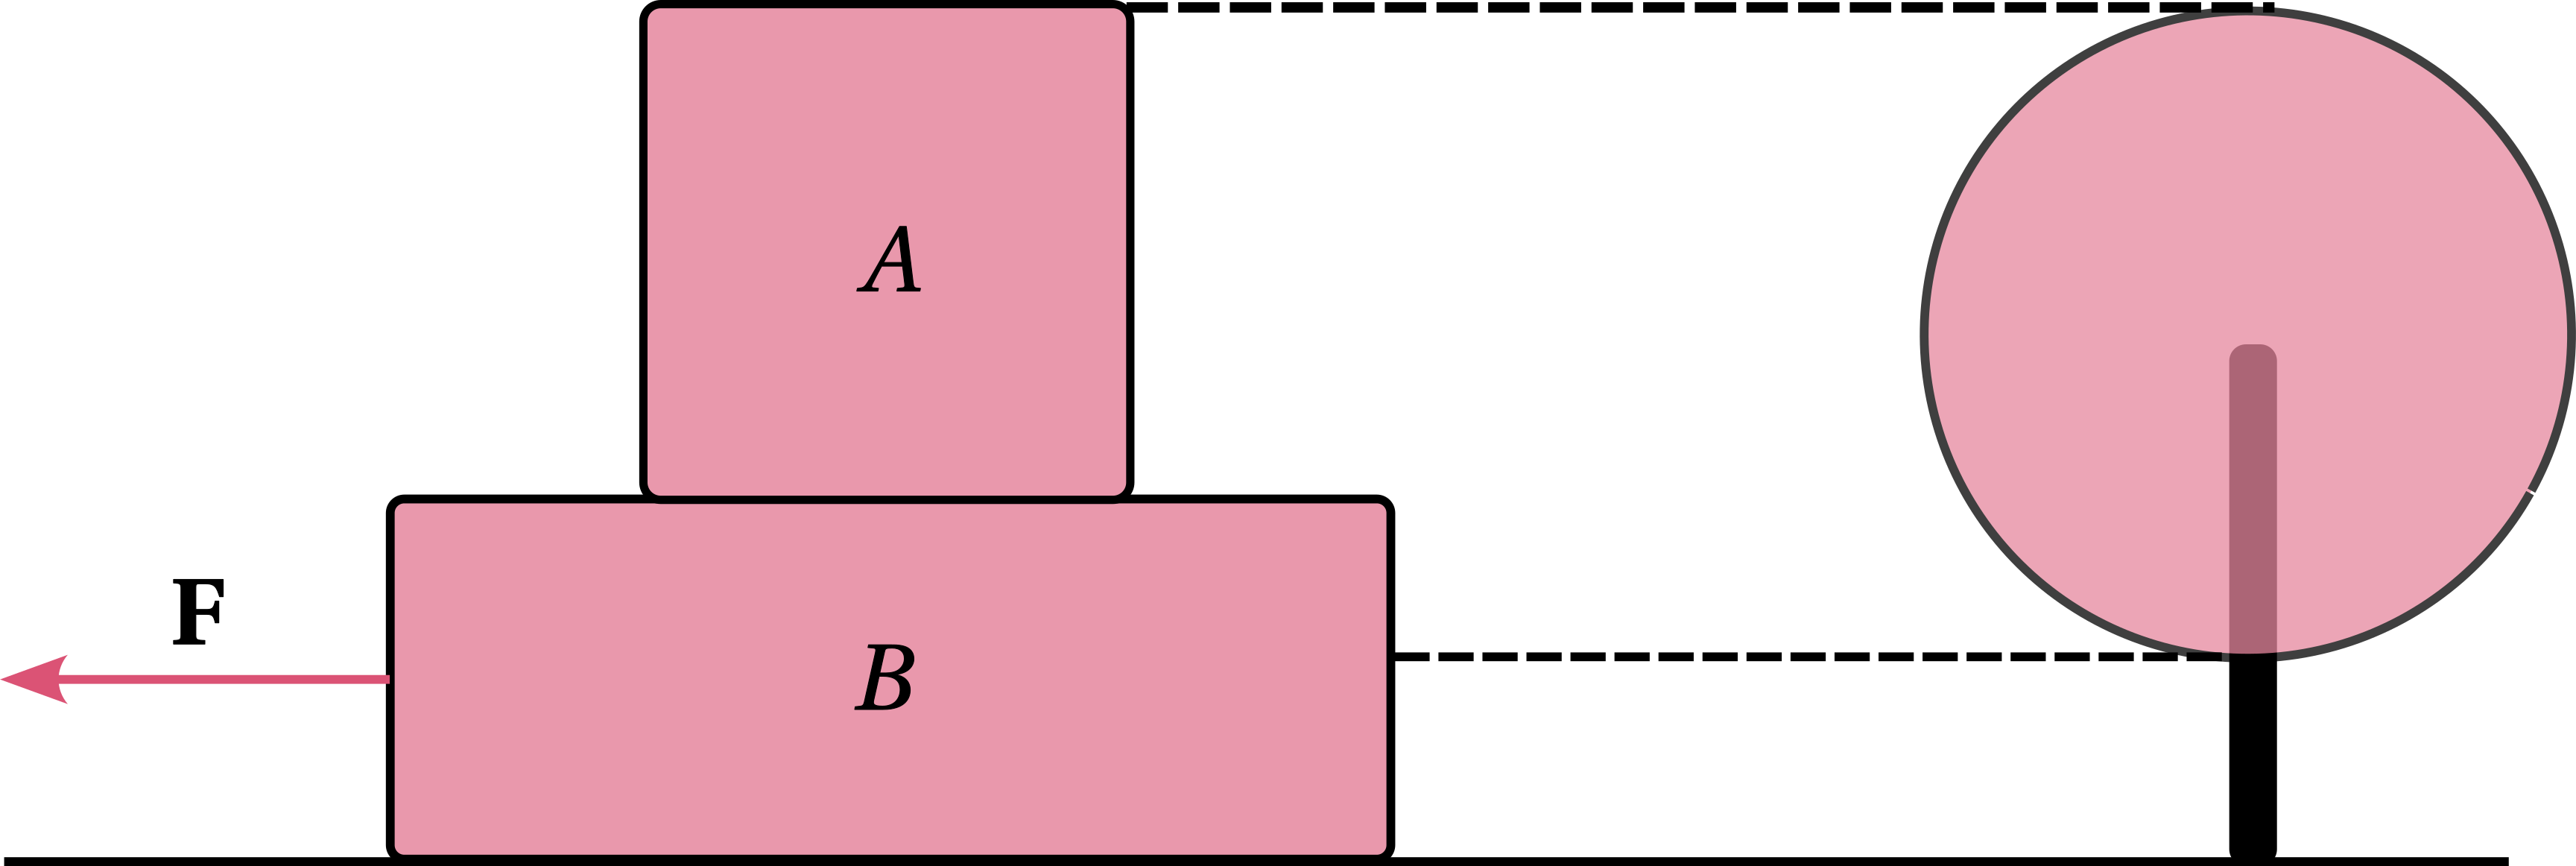
\includegraphics[width=0.53\textwidth]{assets/twoblocks.png}
  \caption{Two blocks and a pulley}
  \label{fig:twoblocks}
\end{wrapfigure}
We take \(+y\) upwards, and \(+x\) rightwards.
We analyse the forces acting on block \(A\) first.
\begin{itemize}
  \item The tension \(\mv{T}\) in the cord acts in the positive \(x\) direction.
  \item The friction by block \(B\) on block \(A\) acts in the
    negative \(x\) direction.
\end{itemize}
Since block \(A\) has zero acceleration, the sum of forces acting on
it must be \(0\).
\begin{equation}
  \mv{T} = \mv{f}_{BA} = \mu \mv{W}_A
  \label{eq:fbdA}
\end{equation}

The forces acting on block \(B\) are more numerous.
\begin{itemize}
  \item The applied force \(\mv{F}\) acts in the negative \(x\) direction.
  \item The friction by block \(A\) on block \(B\) acts to oppose
    this applied force in the positive \(x\) direction.
  \item The friction between the ground and block \(B\) also acts to
    oppose the applied force in the positive \(x\) direction.
  \item The tension \(\mv{T}\) in the cord acts in the positive \(x\) direction.
\end{itemize}
Since the acceleration of block \(B\) is also zero, the sum of forces
acting on it must be zero.
\begin{equation}
  \mv{F} = \mv{f}_{AB} + \mv{f}_B + \mv{T}
  \label{eq:fbdB}
\end{equation}
Substituting \cref{eq:fbdA} into \cref{eq:fbdB},
\begin{align*}
  \mv{F} &= \mv{f}_{AB} + \mv{f}_B + \mv{T} \\
  &= \mv{f}_{AB} + \mv{f}_B + \mv{f}_{BA} \\
  &= \mu\mv{W}_A + \mu\ab(\mv{W}_A + \mv{W}_B) + \mu\mv{W}_A \\
  &= \mu\ab(3\mv{W}_A + \mv{W}_B) \\
  &= \hil{\qty{3.0}{\newton}}
\end{align*}

\section{Rod and trough}
\begin{problem}
  In \cref{fig:rodtrough}, a uniform rod of weight \(\mv{W}\) and
  length \(L\) is supported at its ends by a frictionless trough.
  Show that the centre of gravity of the rod is directly over point \(O\) when
  the rod is in equilibrium.
\end{problem}
\begin{wrapfigure}{o}{0.4\textwidth}
  \centering
  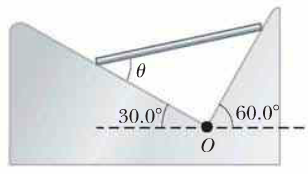
\includegraphics[width=0.38\textwidth]{assets/rodtrough.png}
  \caption{Rod suspended over a trough}
  \label{fig:rodtrough}
\end{wrapfigure}

We first define our variables. Let
\begin{itemize}
  \item the horizontal distance from the left end of the rod to point
    \(O\) be \(d_1\), and the horizontal distance from the right end
    of the rod to point \(O\) be \(d_2\);
  \item the normal contact force exerted by the trough on the left
    end of the rod be \(\mv{F}_1\), and
    that exerted by the trough on the right end of the rod be \(\mv{F}_2\);
  \item the angle the corner of the trough makes with respect to the
    left end be \(\alpha=\qty{30}{\degree}\),
    and that the trough makes with respect to the right end by
    \(\beta=\qty{60}{\degree}\).
\end{itemize}

For the rod to remain in equilibrium, \term{translational equilibrium}
and \term{rotational equilibrium}
must be attained. In translational equilibrium, the \it{vertical}
forces must sum to
zero, i.e. \(\sum\mv{F}_y = 0\).
We obtain the following, taking upwards as \(+y\):
\begin{equation}
  \sum\mv{F}_y = \mv{F}_1\cos\alpha + \mv{F}_2\cos\beta - \mv{W} = 0
  \label{eq:f1f2}
\end{equation}

In rotational equilibrium, the sum of moments about a fixed pivot
must equal \(0\).
We choose \(O\) as the pivot.
Assuming that the centre of gravity is a horizontal distance \(x\)
away from the pivot,
\begin{equation}
  \sum\tau =\mv{F}_1d_1\cos\alpha - \mv{F}_2d_2\cos\beta + \mv{W}x = 0
  \label{eq:f1f2t}
\end{equation}

From \cref{eq:f1f2t}, we learn that
\begin{equation*}
  x = \f{\mv{F}_2d_2\cos\beta - \mv{F}_1d_1\cos\alpha}{\mv{W}}
\end{equation*}

From \cref{eq:f1f2}, we also learn that
\begin{equation*}
  \mv{F}_1 = \f{\mv{W} - \mv{F}_2\cos\beta}{\cos\alpha}
\end{equation*}
Substituting this into the above, we obtain
\begin{align*}
  x &= \f{\mv{F}_2d_2\cos\beta - \mv{F}_1d_1\cos\alpha}{\mv{W}} \\
  &= \f{1}{\mv{W}} \ab(\mv{F}_2d_2\cos\beta -
    \f{\mv{W}-\mv{F}_2\cos\beta}{\cancel{\cos\alpha}}\cdot
  d_1\cancel{\cos\alpha}) \\
  &= \f{1}{\mv{W}} \ab[\ab(d_1+d_2)\mv{F}_2\cos\beta - \mv{W}d_1]
\end{align*}

Notice anything? The expression in \it{square brackets} is the sum of moments
about a new pivot, the left end of the rod! Since the rod is in
rotational equilibrium,
this sum of moments should equal \(0\) as well, causing the rod to stay still.
We can conclude that
\begin{align*}
  x
  &= \f{1}{\mv{W}} \ab[\ab(d_1+d_2)\mv{F}_2\cos\beta - \mv{W}d_1] \\
  &= \f{1}{\mv{W}} \sum\tau \\
  &= \hil{0}
\end{align*}
Since the point at which the weight acts on the rod is a distance of \(x = 0\)
away from \(O\), \hil{the centre of gravity is \it{exactly} above \(O\)}.

\begin{problem}
  Determine the equilibrium value of the angle \(\theta\).
\end{problem}
We let the left end of the rod be denoted by \(X\), and the right end
of the rod be \(Y\).
Since \(\angle XOY=\qty{90}{\degree}\), \(OX=L\cos\theta =
d_1\cos\alpha\) and \(OY =
L\sin\theta=d_2\cos\beta\). Therefore, \(\tan\theta =
\lf{d_2\cos\beta}{d_1\cos\alpha}\).

\section{Wall push}
\begin{problem}
  In \cref{fig:wallpush}, a block of mass \(m = \qty{3.0}{\kg}\) is
  pushed up against a wall by a force
  \(\mv{F}\) that makes an angle \(\theta\) with respect to the horizontal.
  The coefficient of static friction between the block and the wall
  is \(\mu_s\).
  The frictional force acting on the block by the wall is \(\mv{f} =
  \mu_s\mv{R}\),
  where \(\mv{R}\) is the normal contact force acting on the block by the wall.

  Ensuring that the block stays at rest against the wall, what are the minimum
  and maximum values of \(\mv{F}\)?
\end{problem}
\begin{wrapfigure}{o}{0.36\textwidth}
  \centering
  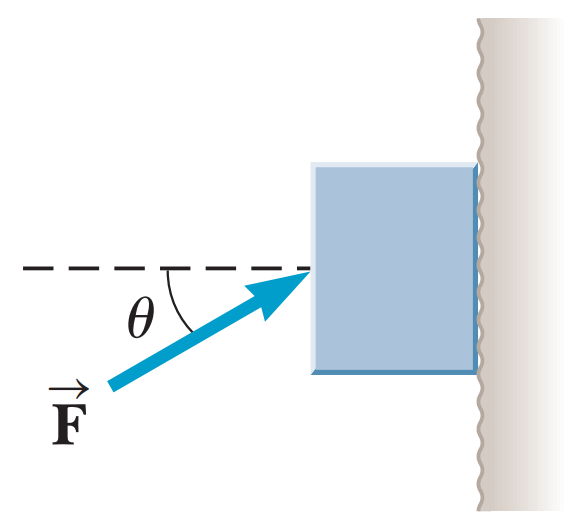
\includegraphics[width=0.35\textwidth]{assets/wallpush.png}
  \caption{Block pushed against wall}
  \label{fig:wallpush}
\end{wrapfigure}
Since the block is in equilibrium, the horizontal and vertical forces should
sum to \(0\).
Taking the sum of the horizontal forces to be \(0\),
\begin{equation}
  \sum\mv{F}_x=\mv{F}\cos\theta-\mv{R}= 0
  \label{eq:fxs}
\end{equation}
Taking the sum of the vertical forces to be \(0\),
\begin{equation}
  \sum\mv{F}_y = \mv{f} + \mv{F}\sin\theta - m\mv{g} = 0
  \label{eq:fys}
\end{equation}
Since \(\mv{f} = \mu_s\mv{R}\), we substitute \cref{eq:fxs} into
\cref{eq:fys} and obtain
\begin{equation}
  \mv{F} = \f{m\mv{g}}{\sin\theta+\mu_s\cos\theta} =
  \f{m\mv{g}}{\sqrt{1+{\mu_s}^2}\sin\ab(\theta+\arctan\mu_s)}
  \label{eq:fmus}
\end{equation}
To find the minimum and maximum values of \(\mv{F}\), we can use
differentiation.
\begin{equation}
  \odv{\mv{F}}{\theta} =
  -m\mv{g}\f{\cos\theta-\mu_s\sin\theta}{\ab(\sin\theta+\mu_s\cos\theta)^2}
  \label{eq:dfd0}
\end{equation}
Finding the zeroes of \(\odv{\mv{F}}{\theta}\) in \cref{eq:dfd0} gives
\begin{align*}
  \cos\theta-\mu_s\sin\theta &= 0 \\
  \sqrt{1+{\mu_s}^2}\cos\ab(\theta+\arctan\mu_s) &= 0
\end{align*}
Therefore, \(\theta_1 = \lf{\pi}{2}-\arctan\mu_s\) and \(\theta_2 =
\lf{3\pi}{2}-\arctan\mu_s\).
Correspondingly, our values of \(\mv{F}\) are:
\begin{align*}
  \mv{F}_1 &= \f{m\mv{g}}{\sqrt{1+{\mu_s}^2}} \\
  \mv{F}_2 &= -\f{m\mv{g}}{\sqrt{1+{\mu_s}^2}}
\end{align*}
Clearly, \hil{\(\mv{F}_1\) is the maximum value and \(\mv{F}_2\) is
the minimum}.

% *** Acids and Bases ***
\chapter{Acids and Bases}
\section{Pre-lesson exercise: Acids and Bases}
\subsection{Acid--base reactions}
\subsubsection{Problem}
Which of the following are \hil{acid--base reactions}
according to the Brønsted--Lowry theory? For the acid--base
reactions in this set, identify the \hil{conjugate acid}
(with its corresponding base\sidenote{A proton-donating substance})
and the \hil[cobalt]{conjugate base} (with its corresponding acid\sidenote{A proton-accepting substance}).

\begin{itemize}
	\item \ch{H2SO4 + H2O -> HSO4- + H3O+}
	\item \ch{(CH3)3N + H2O -> (CH3)3NH^{+} + OH-}
	\item \ch{2 Na + H2O -> 2 NaOH + H2}
	\item \ch{HCl + HCO3- -> Cl- + H2CO3}
	\item \ch{Cl2 + H2 -> 2 HCl}
	\item \ch{CH4 + Cl2 -> CH3Cl + HCl}
\end{itemize}

\subsubsection{Solution}
\begin{itemize}
	\item {\color{accent} \ch{H2SO4 + H2O -> HSO4- + H3O+}}
	      \begin{itemize}
		      \item The acid is \ch{H2SO4}, and its conjugate base is \ch{HSO4-}.
		      \item The base is \ch{H2O}, and its conjugate acid is \ch{H3O+}.
	      \end{itemize}
	\item {\color{accent} \ch{(CH3)3N + H2O -> (CH3)3NH^{+} + OH-}}
	      \begin{itemize}
		      \item The acid is \ch{H2O}, and its conjugate base is \ch{OH-}.
		      \item The base is \ch{(CH3)3N}, and its conjugate acid is \ch{(CH3)3NH^{+}}.
	      \end{itemize}
	\item \ch{2 Na + H2O -> 2 NaOH + H2} is \textbf{not} an acid--base reaction.
	\item {\color{accent} \ch{HCl + HCO3- -> Cl- + H2CO3}}
	      \begin{itemize}
		      \item The acid is \ch{HCl}, and its conjugate base is \ch{Cl-}.
		      \item The base is \ch{HCO3-}, and its conjugate acid is \ch{H2CO3}.
	      \end{itemize}
	\item \ch{Cl2 + H2 -> 2 HCl} is \textbf{not} an acid--base reaction.
	\item {\color{black!40!white} \ch{CH4 + Cl2 -> CH3Cl + HCl}} is a \hil[naples]{disproportionation reaction}.
\end{itemize}

\subsection{Conjugate acids and bases}

\subsubsection{Problem}
Which of the following are
\hil[naples]{conjugate acid--base pairs}\sidenote{Two species that differ by one proton}?

\begin{enumerate}
	\item \ch{CH3CO2H} and \ch{CH3CO2-}
	\item \ch{HCO3-} and \ch{CO3^2-}
	\item \ch{SO3} and \ch{HSO3-}
	\item \ch{[Al(H2O)6]^3+} and \ch{[Al(H2O)5(OH)]^2+}
	\item \ch{BH3} and \ch{BH4-}
	\item \ch{H-} and \ch{H2}
\end{enumerate}
\subsubsection{Solution}
\begin{itemize}
	\item {\color{accent} \ch{CH3CO2H} and \ch{CH3CO2-}} are a conjugate acid--base pair.
	\item {\color{accent} \ch{HCO3-} and \ch{CO3^2-}} are a conjugate acid--base pair.
	\item \ch{SO3} and \ch{HSO3-} are \textbf{not} a conjugate acid--base pair.
	\item {\color{accent} \ch{[Al(H2O)6]^3+} and \ch{[Al(H2O)5(OH)]^2+}} are a conjugate acid--base pair.
	\item \ch{BH3} and \ch{BH4-} are \textbf{not} a conjugate acid--base pair.
	\item {\color{accent} \ch{H-} and \ch{H2}} are a conjugate acid--base pair.
\end{itemize}

% *** homework ***
\pagebreak
\section{Homework: Acids and Bases}
\subsection{Polyprotic acids}
\subsubsection{Problem}
In a \hil{polyprotic acid} \sidenote{A substance capable of donating more than one proton},
we have successive \(\Ka\) values for each successive
dissociation. For example, phosphoric acid has three dissociations, and so has
correspondingly three \(\Ka\) values, one for each dissociation (Equations~\ref{eq:polyprotic}):
\begin{align*}
	\ch{H3PO4 \aq{}     & <=> H^{+} \aq{} + H2PO4- \aq}    \\%\nonumber            \\
	\ch{H2PO4- \aq{}    & <=> H^{+} \aq{} + HPO4^{2-} \aq} \\%\nonumber            \\
	\ch{HPO4^{2-} \aq{} & <=> H^{+} \aq{} + PO4^{3-} \aq}
	\label{eq:polyprotic}
\end{align*}

The corresponding \Ka\ values are
\begin{align*}
	K_1 & = \num{7.11e-3}  \\
	K_2 & = \num{6.32e-8}  \\
	K_3 & = \num{4.48e-13}
\end{align*}

\begin{enumerate}
	\item\label{item:decreased-ka} Suggest why, for most polyprotic acids, the successive \(\Ka\) values
	      will decrease by a large factor.
	\item\label{item:significance} \bf{Assuming only the first dissociation of phosphoric acid is significant},
	      calculate the \pH\ of \qty{0.0750}{\conc} phosphoric acid.
	\item Based on your answer to Part~\ref{item:decreased-ka}, estimate \ch{[H3PO4]},
	      \ch{[H2PO4^{-}]}, \ch{[HPO4^{2-}]} and \ch{[PO4^{3-}]} in the phosphoric acid
	      solution. From your calculations, is the assumption in Part~\ref{item:significance}
	      valid?
\end{enumerate}

\subsubsection{Solution}
It becomes more difficult for polyprotic acids to lose \ch{H+} ions with each
dissociation, since {\color{accent} \ch{H+} ions are less likely to leave an increasingly
		negatively-charged anion}.
\begin{equation*}
	K_1 = \frac{\ch{[H^{+}]} \ch{[H2PO4^{-}]}}{\ch{[H3PO4]}}
\end{equation*}
We can construct an ICE table, where \(x\) is the change in concentration of
each species (Table~\ref{tab:h3po4}).
\begin{table}[htpb]
	\centering
	\begin{tabular}{l r r r}
		\toprule
		\textbf{Concentration / \unit{\conc}} & \ch{H3PO4}           & \ch{H+} & \ch{H2PO4^{-}} \\
		\midrule
		Initial                               & \num{0.0750}         & 0       & 0              \\
		Change                                & \(-x\)               & \(+x\)  & \(+x\)         \\
		End                                   & \(\num{0.0750} - x\) & \(x\)   & \(x\)          \\
		\bottomrule
	\end{tabular}
	\caption{ICE table for the dissociation of \ch{H3PO4}}
	\label{tab:h3po4}
\end{table}

Hence, by assuming that only the dissociation of \ch{H3PO4} is significant,
\begin{align*}
	\num{7.11e-3} & = \f{x^2}{\num{0.0750} - x}  \\
	x             & = \qty{1.981e-2}{\conc}      \\
	\pH           & = -\lg x                     \\
	              & = \color{accent} \num{1.703}
\end{align*}

Hence,
\begin{align*}
	\ch{[H3PO4]}   & \approx 0.0750 - x     \\
	               & = \qty{0.05519}{\conc} \\
	\ch{[H2PO4^-]} & \approx x              \\
	               & = \qty{0.01981}{\conc}
\end{align*}

Let \(y\) be \ch{[HPO4^{2-}]} formed by the second dissociation.
\begin{align*}
	K_2 & = \f{\ch{[H^+]} \ch{[HPO4^{2-}]}}{\ch{[H2PO4^-]} - y} \\
	    & = \f{y \ab(y + \num{0.01981})}{\num{0.01981} - y}     \\
	y   & = \qty{6.3e-8}{\conc}
\end{align*}

Since \(y\) is minuscule compared to \(x\), the assumption in
Part~\ref{item:significance} can be accepted.

Let \(z\) be \ch{[PO4^{3-}]} formed by the third dissociation.
\begin{align*}
	K_3 & = \f{\ch{[H^+]} \ch{[PO4^{3-}]}}{\ch{[H2PO4^-]} - z} \\
	    & = \f{z \ab(z + \num{0.01981})}{y-z}                  \\
	z   & \approx 0
\end{align*}
Since \(z \approx 0\), the assumption in
Part~\ref{item:significance} can be accepted for the third dissociation also.

\subsection{Titration curves}
\subsubsection{Problem}
Sketch the titration curve of \ch{H2SO3}, a diprotic weak acid, against
\ch{NaOH} \sidenote{\ch{NaOH} is a strong base.}.
Suggest the indicators you would add in order to see both end points clearly, and
state their colour changes.

\subsubsection{Solution}
\ch{H2SO3} dissociates according to the following equations:
\begin{align*}
	\ch{H2SO3 \aq{}  & <=> HSO3^- \aq{} + H^+ \aq}   \\
	\ch{HSO3^- \aq{} & <=> SO3^{2-} \aq{} + H^+ \aq}
\end{align*}
Since \ch{H2SO3} is a weak acid, the increase in \pH\ will be more gradual
than those expected with a strong acid.
\begin{figure}[htpb]
	\centering
	\begin{tikzpicture}
		\begin{axis}[ticks=none, xlabel={Volume of \ch{NaOH} added}, ylabel={pH}]
			% Adding points manually based on assumed calculations
			\addplot[
				smooth,
			] coordinates {
					% step 1
					(0, 1.9) (5, 1.93) (10, 1.95) (15, 1.975)
					(20, 2) (22, 2.1) (24, 2.25) (26, 2.35)
					(28, 2.4) (30, 2.5) (32, 2.7) (34, 2.9)
					(36, 3.2) (38, 3.5) (39, 3.75) (40, 4)
					% step 2
					(42, 4.5) (44, 5) (46, 5.5) (48, 6) (50, 6.2)
					(52, 6.4) (54, 6.6) (56, 6.8) (58, 6.9) (59, 6.95)
					(60, 7) (61, 7.05) (62, 7.07) (63, 7.1) (65, 7.15)
					(67, 7.2) (68, 7.22) (70, 7.24) (72, 7.51) (74, 7.82)
					(76, 8.44) (78, 8.87) (79, 9.5) (80, 10) (82.5, 10.5)
					(85, 11) (87.5, 11.5) (89, 12) (90, 12) (95, 12) (97, 12)
					(100, 12) (105, 12) (110, 12) (115, 12) (118, 12) (120, 12)
				};
			\addplot+ [only marks] coordinates {
					(40, 4) (80, 10)
				};
		\end{axis}
	\end{tikzpicture}
	\caption{Titration curve of \ch{H2SO3} with \ch{NaOH}}
	\label{fig:titration-h2so3}
\end{figure}

The titration curve is in Figure~\ref{fig:titration-h2so3}. We can use {\color{accent}
		methyl orange} for the first endpoint, and {\color{accent} phenolphthalein} for the second.

\subsection{Liquid--liquid extraction}
\subsubsection{Problem}
Liquid--liquid extraction (Figure~\ref{fig:ll-sep}) is a technique to separate
organic compounds using a separatory funnel. The crude sample is first dissolved
in an organic solvent such as hexane and this solution is poured into a separatory funnel.
Next, water is added to the separatory funnel and the funnel is shaken.
Because hexane and water are immiscible, they form two layers in the
separatory funnel. The organic compound that is more soluble in water will migrate
from the hexane layer to the water layer. The two layers contain different
compounds and can be collected separately.

\begin{wrapfigure}{r}{0.5\textwidth}
	\centering
	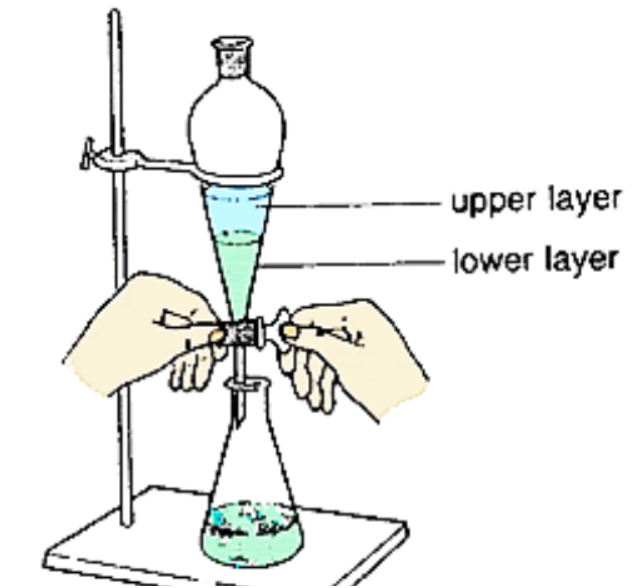
\includegraphics[width=0.5\linewidth]{assets/08_ll_separation.png}
	\caption{Liquid--liquid separation}
	\label{fig:ll-sep}
\end{wrapfigure}

You are given a sample containing both phenol (\(\pKa = \num{9.95}\)) and benzoic
acid (\(\pKa = \num{4.20}\)). Both compounds are not very soluble in water. To
improve the separation, aqueous sodium bicarbonate (\ch{NaHCO3}) can be used instead
of water.

It is given that \(\pKa_1 = \num{6.3}\) and \(\pKa_2 = \num{10.3}\) for carbonic
acid, \ch{H2CO3}. In which layer will the majority of the benzoic acid be found?
In which layer will the majority of the phenol be found? You need not perform
equilibrium computations.

\subsubsection{Solution}
\ch{NaHCO3} is a weak base. We can write
\begin{equation*}
	\ch{HCO3^- \aq{} <=> CO3^{2-} \aq{} + H^+ \aq}
\end{equation*}
We can also write the dissociation of \ch{H2CO3 \aq} as
\begin{align*}
	\ch{H2CO3 \aq{}    & <=> HCO3^{-} \aq{} + H^+ \aq} \\
	\ch{HCO3^{-} \aq{} & <=> CO3^{2-} \aq{} + H^+ \aq}
\end{align*}
It is the \it{second} dissociation of \ch{H2CO3 \aq} we desire. We use
\(\pKa \coloneqq \pKa_2 = \num{10.3}\).

Since the \pKa\ of benzoic acid (\num{4.20}) is smaller than that of phenol
(\num{9.95}), it has a larger \Ka\ and hence is the stronger acid. It will react
more readily with the \ch{NaHCO3 \aq} to form benzoate ions, which are soluble
in water. {\color{accent} The majority of the benzoic acid will be found in the
		aqueous layer.}

On the other hand, the \pKa\ values of phenol and \ch{H2CO3 \aq} are closer
to each other, making the acid--base reaction less favourable. {\color{accent}
		Phenol will predominantly be found in the hexane layer.}


\chapter{Electrochemistry}

\section{Pre-lesson exercise: Electrochemistry}
\subsection{Metals}
\subsubsection{Problem}
\bf{W}, \bf{X}, \bf{Y} and \bf{Z} are four unknown metals.

\bf{Y} does not react with water.

Precipitation is observed when solid \bf{W} is added into a solution of \bf{Z}
chloride.  No visible change is observed when solid \bf{W} is added into a solution
of \bf{Y} chloride.

Based on the above information, match the following metals to the correct
letters:
\begin{itemize}
	\item \ch{Mg}
	\item \ch{Al}
	\item \ch{Fe}
	\item \ch{Cu}
\end{itemize}

\subsubsection{Solution}

Since \bf{W} displaces \bf{Z} but not \bf{Y}, \bf{W} is more reactive than \bf{Z}
but less reactive than \bf{Y}. However, \bf{Y} does not react with water,
indicating that it is not highly reactive.

We can conclude that:
\begin{itemize}
	\item {\color{accent} \bf{W} is iron}. It has a reactivity in between that of two metals.
	\item {\color{accent} \bf{Z} is copper}. It has the lowest reactivity, since \bf{W} could displace it.
	\item {\color{accent} \bf{Y} is aluminium}. It is more reactive than \bf{W}, yet cannot dissolve in water, indicating that its reactivity is not the highest.
	\item {\color{accent} \bf{X} is, therefore, magnesium}.
\end{itemize}

\subsection{Electrolysis}
\subsubsection{Problem}
The electrolysis of dilute sodium nitrate was conducted as shown in Figure~\ref{fig:electrolysis-nano3}.
\begin{figure}[htpb]
	\centering
	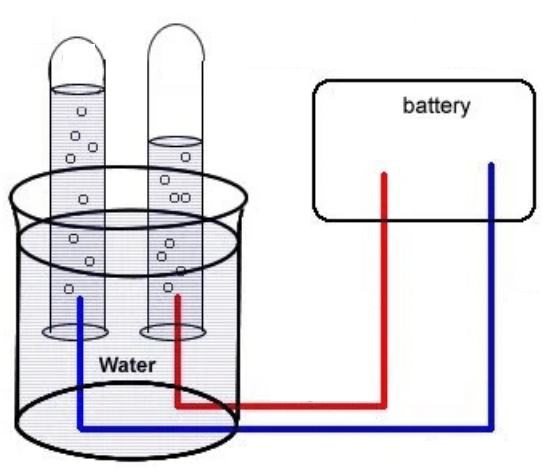
\includegraphics[width=0.4\linewidth]{assets/09_electrolysis_nano3.png}
	\caption{Electrolysis of \ch{NaNO3 \aq}}
	\label{fig:electrolysis-nano3}
\end{figure}
\begin{enumerate}
	\item\label{part:no3-discharge} With reference to oxidation numbers, explain why the nitrate anion will not be discharged.
	\item\label{part:na-discharge} Explain why the sodium cation will not be discharged.
	\item Despite Parts~\ref{part:no3-discharge} and~\ref{part:na-discharge}, explain why
	      the electrolysis will not work without sodium nitrate.
	\item By considering the oxidation and reduction reactions taking place, label the following on the diagram:
	      \begin{itemize}
		      \item the polarity of the battery (\(+\) or \(-\)),
		      \item the anode and the cathode, and
		      \item the flow of electrons, and the flow of electrical current.
	      \end{itemize}
	\item State what will be observed when a few drops of universal \pH\ indicator
	      are added into the solution.
\end{enumerate}

\subsubsection{Solution}
\ch{N} in \ch{NO3^-} has an oxidation state of \(+5\). Since \ch{N} is in
group 15 in the periodic table, \(+5\) is its maximum oxidation state. Since \ch{NO3^-}
is an anion, one would expect it to be oxidised at the anode. However, the
oxidation of \ch{NO3^-} is defined as the increase in oxidation state of \ch{N},
which is impossible. Therefore, \ch{NO3^-} cannot be oxidised.

The competing species at the cathode (to be reduced) are \ch{Na^+} and \ch{H2O}, since the electrolyte
is an aqueous solution. \ch{H2O}, however, is lower in the electrochemical series,
so it is preferentially reduced over \ch{Na^+}. The reduction of \ch{H2O}
forms \ch{H2 \gas{}}, and the reduction of \ch{Na^+} will only take place once
all \ch{H2O} has been reduced/oxidised.

Without \ch{NaNO3 \aq}, only \ch{H2O \lqd} would be present in the electrolyte.
Assuming that \ch{H2O \lqd} is deionised for the purposes of this electrolysis, it
will not allow electron flow without mobile ions which act as mobile charge carriers.

The annotated diagram is in Figure~\ref{fig:nano3-ans}.

\begin{figure}[htpb]
	\centering
	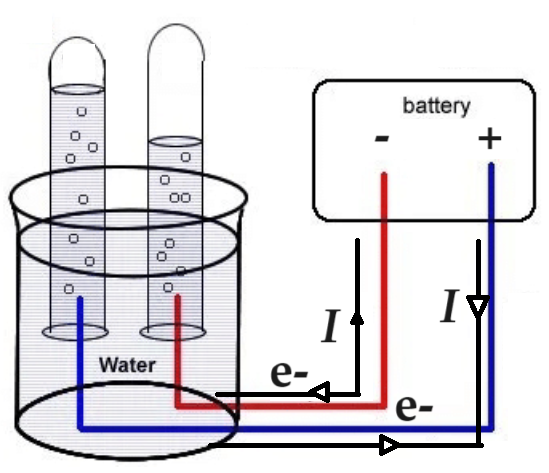
\includegraphics[width=0.4\linewidth]{assets/09_electrolysis_nano3_ans.png}
	\caption{Annotated electrolysis diagram}
	\label{fig:nano3-ans}
\end{figure}

\ch{H2O \lqd} is both preferentially reduced and oxidised at the cathode and anode
respectively.
\begin{align*}
	\ch{2 H2O \lqd{} + 2 e- & <=> H2 \gas{} + 2 OH^- \aq}             \\
	\ch{H2O \lqd{}          & <=> 1/2 O2 \gas{} + 2 H^+ \aq{} + 2 e-}
\end{align*}
For the same number of moles of electrons passed through the electrolyte, the
number of moles of \ch{OH^-} and \ch{H^+} produced are equal. The overall \pH\
of the solution does not change.

However, \ch{H^+} ions are produced at the anode, meaning that the solution surrounding
the anode will turn {\color{accent} acidic}. {\color{accent} Near the anode, the green universal
\pH\ indicator will turn red}.

\ch{OH^-} ions are produced at the cathode, meaning that the solution surrounding
the cathode will turn {\color{cobalt} basic}. {\color{cobalt} Near the cathode, the green universal \pH\ indicator will turn purple.}

% *** *** ***
\section{Homework: Electrochemistry}

\subsection{Electrochemical cells}
\subsubsection{Problem}
A \bf{standard} electrochemical cell is prepared involving two reactions: the
oxidation of sodium sulfate into sodium peroxydisulfate (\ch{Na2S2O8}) and the
reduction of iron(III) chloride into iron(II) chloride. Write down the cell
reaction for the above cell.

Given the following \(E^\standardstate\) values, determine if the following
statements are true or false.

\begin{align*}
	\ch{S2O8^{2-} \aq{} + 2 e- <=> 2 SO4^{2-} \aq} & \quad E^\standardstate = +\qty{2.05}{\volt} \\
	\ch{Fe^{3+} \aq{} + e- <=> Fe^{2+} \aq}        & \quad E^\standardstate = +\qty{0.77}{\volt}
\end{align*}

\begin{enumerate}
	\item The equilibrium constant of the cell reaction is very small.
	\item If the platinum foils are connected directly, the colour of the \ch{"\ox{2,Fe}"}/\ch{"\ox{3,Fe}"} solution
	      intensifies.
	\item When connected in the conventional way, this cell cannot light up an LED bulb.
	\item If we mix aqueous iron(III) sulfate with potassium persulfate (\ch{K2S2O8}), the solution will
	      turn from yellow to pale green.
	\item Swapping the two half-cells around generates a battery of voltage \qty{1.28}{\volt}.
\end{enumerate}

\subsubsection{Solution}
The cell reaction \sidenote{A combination of the two half-reactions.} is
\begin{equation*}
	\ch{2 SO4^{2-} \aq{} + 2 Fe^{3+} \aq{} -> S2O8^{2-} \aq{} + 2 Fe^{2+} \aq}
\end{equation*}

If a reaction has a small equilibrium constant, the equilibrium position favours
the reactants. The products do not form spontaneously. At the same time,
\begin{align*}
	E^\standardstate_\text{cell} & = E^\standardstate_\text{cathode} - E^\standardstate_\text{anode} \\
	                             & = 0.77 - 2.05                                                     \\
	                             & = \qty{-1.28}{\volt}                                              \\
	                             & < 0
\end{align*}
\(E^\standardstate_\text{cell} < 0\) confirms that the reaction is not spontaneous.
Therefore, it is {\color{accent} true} that the reaction has a small equilibrium
constant.

If the platinum electrodes are connected directly, the circuit will be shorted.
Since \(E_\text{cell} = E^\standardstate_\text{cell} < 0\), electrons will flow
in the opposite direction and the reverse of the cell reaction occurs. \ch{Fe^{3+} \aq}
will be formed from \ch{Fe^{2+} \aq}, so it is {\color{accent} true} that the colour of the solution
intensifies to a deeper yellow-orange as \ch{[Fe^{3+}]} increases.

Since \(E_\text{cell} < 0\), electrons cannot flow in the cell when connected
conventionally. Therefore, it is {\color{accent} true} that an LED bulb cannot
light up.

Since the equilibrium position favours the reaction's reactants and not its
products, the increased concentration of \ch{S2O8^{2-} \aq} will hinder
the rate of reaction of \ch{SO4^{2-} \aq} and \ch{Fe^{3+} \aq} further.
It is unlikely that a large amount of \ch{Fe^{3+} \aq} will be used up, and
therefore {\color{accent} untrue} that the yellow colour of \ch{Fe^{3+} \aq}
will turn into the pale-green colour of \ch{Fe^{2+} \aq}.

Swapping the two electrodes causes the reverse reaction to occur. The reverse
reaction occurs more readily and electrons will flow in the opposite direction,
producing a battery whose voltage is the negative of the cell potential, i.e.
\qty{1.28}{\volt}.

\subsection{Spontaneous reactions}
\subsubsection{Problem}
A list of values (in alphabetical order) is provided below. Use the relevant values to
determine if a reaction is spontaneous and write a balanced equation for those reactions
which are spontaneous.

\begin{alignat*}{3}
	\ch{Ag+ \aq{} + \el{}                   & <=> Ag \sld} \quad                  & E^\standardstate & = +\qty{0.80}{\volt} \\
	\ch{Cl2 \gas{} + 2 \el{}                & <=> 2 Cl- \aq} \quad                & E^\standardstate & = +\qty{1.36}{\volt} \\
	\ch{ClO2^- \aq{} + H2O \lqd{} + 2 \el{} & <=> ClO- \aq{} + 2 OH- \aq} \quad   & E^\standardstate & = +\qty{0.59}{\volt} \\
	\ch{Fe^2+ \aq{} + 2 \el{}               & <=> Fe \sld} \quad                  & E^\standardstate & = \qty{-0.44}{\volt} \\
	\ch{Fe^3+ \aq{} + 3 \el{}               & <=> Fe \sld} \quad                  & E^\standardstate & = \qty{-0.04}{\volt} \\
	\ch{Fe^3+ \aq{} + \el{}                 & <=> Fe^2+ \aq} \quad                & E^\standardstate & = +\qty{0.77}{\volt} \\
	\ch{Fe(OH)3 \sld{} + \el{}              & <=> Fe(OH)2 \sld{} + OH- \aq} \quad & E^\standardstate & = \qty{-0.56}{\volt} \\
	\ch{I2 \sld{} + 2 \el{}                 & <=> 2 I- \aq} \quad                 & E^\standardstate & = +\qty{0.54}{\volt} \\
	\ch{Na+ \aq{} + \el{}                   & <=> Na \sld} \quad                  & E^\standardstate & = \qty{-2.71}{\volt} \\
	\ch{NO3^- \aq{} + 2 H+ \aq{} + \el{}    & <=> NO2 \gas{} + H2O \lqd} \quad    & E^\standardstate & = +\qty{0.81}{\volt} \\
	\ch{SO4^2- \aq{} + 4 H+ \aq{} + 2 \el{} & <=> SO2 \gas{} + 2 H2O \lqd} \quad  & E^\standardstate & = +\qty{0.17}{\volt} \\
\end{alignat*}

\begin{enumerate}
	\item Mixing aqueous iron(III) sulfate with acidified aqueous iron(II) sulfate
	\item Bubbling chlorine gas through alkaline aqueous sodium chlorate(I)
	\item Reducing iron(III) hydroxide with aqueous potassium iodide
	\item Dropping an iron nail into aqueous iron(III) chloride
	\item Dropping silver into concentrated nitric acid
\end{enumerate}

\subsubsection{Mixing aqueous iron(III) sulfate with acidified aqueous iron(II) sulfate}
The cell reaction is
\begin{equation*}
	\ch{Fe^3+ \aq{} + Fe^2+ \aq{} -> Fe^2+ \aq{} + Fe^3+ \aq}
\end{equation*}
where \ch{Fe^3+ \aq} had been reduced and \ch{Fe^2+ \aq} had been oxidised.
Therefore,
\begin{align*}
	E^\standardstate_\text{cell} & = +0.77 - (+0.77)   \\
	                             & = \qty{0.00}{\volt}
\end{align*}
The reaction mixture is {\color{accent} in equilibrium} under standard conditions.

\subsubsection {Bubbling chlorine gas through alkaline aqueous sodium chlorate(I)}
The cell reaction is
\begin{equation*}
	\ch{ClO- \aq{} + Cl2 \gas{} + 2 OH- \aq{} -> ClO2^- \aq{} + 2 Cl- \aq{} + H2O \lqd{} + 2 \el}
\end{equation*}
and
\begin{align*}
	E^\standardstate_\text{cell} & = +1.36 - (-0.59)       \\
	                             & = \qty{1.95}{\volt} > 0
\end{align*}
The reaction is {\color{accent} spontaneous}.

\subsubsection {Reducing iron(III) hydroxide with aqueous potassium iodide}
The cell reaction is
\begin{equation*}
	\ch{2 Fe(OH)3 \sld{} + 2 I- \aq{} -> 2 Fe(OH)2 \sld{} + I2 \lqd{} + 2 OH- \aq}
\end{equation*}
and
\begin{align*}
	E^\standardstate_\text{cell} & = -0.56 - (-0.54)        \\
	                             & = \qty{-0.02}{\volt} < 0
\end{align*}
The reaction is {\color{accent} not spontaneous}, but its reverse is under
standard conditions.

\subsubsection{Dropping an iron nail into aqueous iron(III) chloride}
The cell reaction is \sidenote{This is a synproportionation!}
\begin{equation*}
	\ch{Fe \sld{} + 2 Fe^3+ \aq{} -> 3 Fe^2+ \aq}
\end{equation*}
and
\begin{align*}
	E^\standardstate_\text{cell} & = +0.77 - \ab(+0.44)     \\
	                             & = +\qty{0.33}{\volt} > 0
\end{align*}
The reaction here is {\color{accent} spontaneous}.

\subsubsection{Dropping silver into concentrated nitric acid}

The cell reaction is
\begin{equation*}
	\ch{Ag \sld{} + NO3^- \aq{} + 2 H+ \aq{} ->  Ag+ \aq{} + NO2 \gas{} + H2O \lqd}
\end{equation*}
and
\begin{align*}
	E^\standardstate_\text{cell} & = +0.81 - \ab(-0.80)     \\
	                             & = +\qty{1.61}{\volt} > 0
\end{align*}
The reaction here is {\color{accent} spontaneous}.

\subsection{Calculations}
\subsubsection{Problem}
\begin{enumerate}
	\item Calculate the time needed for a constant current of \qty{1.20}{\ampere} to produce
	      \qty{0.500}{\gram} of elemental thallium on a cathode, from a solution of \ch{"\ox{1,Tl}"}
	      ions.

	\item Under suitable conditions, we can deposit the oxide \ch{Co3O4} on an anode
	      from the electrolysis of a \ch{"\ox{2,Co}"} source. Calculate the minimum current
	      required to deposit \qty{2.00}{\gram} of the oxide on the anode within \qty{1}{\hour}.

	\item \qty{.2416}{\gram} of a water-insoluble, monoprotic carboxylic acid was measured out
	      and mixed with a concentrated sodium chloride solution with constant stirring. After
	      electrolysing the concentrated solution for \qty{5.40}{\minute} with a constant current
	      of \qty{367}{\milli\ampere}, all the organic acid dissolved. Determine the molar mass
	      of the acid and suggest a possible structure.
\end{enumerate}

\subsubsection{Solution: Thallium deposition}
We can write the reduction of \ch{"\ox{1,Tl}"} as
\begin{equation*}
	\ch{Tl+ \aq{} + \el{} -> Tl \sld}
\end{equation*}
where one mole of electrons is required for one mole of solid thallium to be deposited.
\begin{align*}
	\eta_{ \el{} } = \eta_{ \ch{Tl+} } & = \f{ \qty{0.500}{\gram} }{ \qty{204.4}{\gram\per\mol} }                                     \\
	                                   & = \qty{2.446e-3}{\mol}                                                                       \\
	\\
	n_{ \el{} }                        & = \ab( \qty{2.446e-3}{\mol} ) \times \ab( \qty{6.02e23}{\per\mol} )                          \\
	                                   & = \num{1.473e21}                                                                             \\
	\\
	\because\; Q = It                  & = ne                                                                                         \\
	\therefore\; t                     & = \f{ne}{I}                                                                                  \\
	                                   & = \f{ \ab( \num{1.473e21} ) \times \ab( \qty{1.602e-19}{\coulomb} ) }{ \qty{1.20}{\ampere} } \\
	                                   & = \color{accent} \qty{196.6}{\second}
\end{align*}

\subsubsection{Solution: Cobalt oxide??}
\begin{align*}
	\eta_{ \ch{Co3O4} } & = \f{ \num{2.00} }{ 58.9 \times 3 + 16.0 \times 4 } \\
	                    & = \qty{ 8.309e-3 }{ \mol }                          \\
\end{align*}
We can write the oxidation of \ch{"\ox{2,Co}"} into \ch{Co3O4} as
\begin{equation*}
	\ch{3 Co^2+ \aq{} + 4 H2O \lqd{} -> Co3O4 \sld{} + 8 H+ \aq{} + 2 \el{}}
\end{equation*}
For every mole of \ch{Co3O4} deposited, \qty{2}{\mol} of electrons are passed.
\begin{align*}
	\eta_{ \el{} } & = \ab(\qty{8.309e-3}{\mol}) \times 2                                          \\
	n_{ \el{} }    & = \ab[\ab(\qty{8.309e-3}{\mol}) \times 2] \times \ab(\qty{6.02e23}{\per\mol}) \\
	               & = \num{1.000e22}
\end{align*}
We can do something similar to what we've done previously.
\begin{align*}
	\because \; Q = It & = ne                                                                                                        \\
	\therefore \; I    & = \f{ne}{t}                                                                                                 \\
	                   & = \f{ \ab(\num{1.000e22}) \times \ab( \qty{1.602e-19}{\coulomb} ) }{ 1 \times 60 \times \qty{60}{\second} } \\
	                   & = \color{accent} \qty{4.45}{\deci\ampere}
\end{align*}

\subsubsection{Solution: Organic chemistry (again)}
We have to work backwards. Let's start by finding the amount of electrons passed.
\begin{align*}
	\because \; Q = I t & = n e                                                                                                                                   \\
	\therefore \; n     & = \f{I t}{e}                                                                                                                            \\
	                    & = \f{ \ab( \qty{367e-3}{\ampere} ) \times \ab( \qty{5.40}{\minute} \times \qty{60}{\second\per\minute} ) }{ \qty{1.602e-19}{\coulomb} } \\
	                    & = \num{7.422e20}                                                                                                                        \\
	\eta_{ \el{} }      & = \f{ \num{7.422e20} }{ \qty{6.02e23}{\per\mol} }                                                                                       \\
	                    & = \qty{1.233e-3}{\mol}
\end{align*}
The electrolysis of concentrated sodium chloride solution (or brine) can be written as
\begin{align*}
	\ch{2 H2O \lqd{} + 2 \el{} & -> H2 \gas{} + 2 OH- \aq} \\
	\ch{2 Cl- \aq{}            & -> Cl2 \gas{} + 2 \el}    \\
\end{align*}
For every \qty{2}{\mol} of \ch{OH- \aq} produced, \qty{2}{\mol} of electrons
were passed. The \ch{OH- \aq} were crucial in neutralising the carboxylic acid.
\begin{align*}
	\eta_{ \ch{OH-} } & = \eta_{ \el{} }       \\
	                  & = \qty{1.233e-3}{\mol}
\end{align*}
Let the carboxylic acid be \ch{R-COOH}. Since the acid had been completely
neutralised, \( \eta_{ \ch{H+} } = \eta_{ \ch{OH-} } \).
\begin{align*}
	\eta_{ \ch{R-COOH} }   & = \eta_{ \ch{OH-} }                                       \\
	                       & = \qty{1.233e-3}{\mol}                                    \\
	M_r                    & = \f{ \qty{.2416}{\gram} }{ \qty{1.233e-3}{\mol} }        \\
	                       & = \color{accent} \qty{195.95}{\gram\per\mol}              \\
	M_r \text{ of \ch{R} } & = \qty{195.95}{\gram\per\mol} - \qty{45.0}{\gram\per\mol} \\
	                       & = \qty{150.95}{\gram\per\mol}
\end{align*}

\chapter{Inorganic Chemistry}
\section{Pre-lesson Exercise: Inorganic Chemistry}
\subsection{Balanced equations}
\subsubsection{Problem}
Write balanced equations to account for the following observations.
\begin{enumerate}
	\item When excess \ch{NaOH \aq} is added to a solution of lead(II) nitrate, a
	      white precipitate is observed. This precipitate dissolves when dilute \ch{HNO3}
	      is added, but not when dilute \ch{HCl} is added.
	\item The addition of \ch{NaOH \aq} to a pale green-coloured solution gives a dirty
	      green precipitate, which turns brown after a few minutes.
	\item The addition of hot \ch{NaOH \aq} to a colourless solution resulted in the
	      evolution of a pungent alkaline gas.
	\item The addition of \ch{HCl \aq} to a zinc salt resulted in the effervescence
	      of a gas, which when bubbled into limewater formed a white precipitate. Upon further
	      bubbling, the white precipitate dissolved.
\end{enumerate}

\subsubsection{Excess sodium hydroxide and lead(II) nitrate}
\begin{align*}
	\ch{2 NaOH \aq{} + Pb(NO3)2 \aq{}       & -> \hil{Pb(OH)2} \sld{} + 2 NaNO3 \aq} \\
	\ch{\hil{Pb(OH)2} \sld{} + 2 HNO3 \aq{} & -> Pb(NO3)2 \aq{} + 2 H2O \lqd}        \\
\end{align*}
However,
\begin{equation*}
	\ch{\hil{Pb(OH)2} \sld{} + 2 \bf{HCl} \aq{} -> PbCl2 \sld{} + 2 H2O \lqd}        \\
\end{equation*}
\ch{PbCl2} is insoluble in water, whereas \ch{Pb(NO3)2} is \sidenote{All nitrates are!}.

\subsubsection{Sodium hydroxide and the green solution}
We can identify the cation in the \hil[green!50!black]{solution} as \ch{Fe^2+}.
\begin{equation*}
	\ch{Fe^2+ \aq{} + NaOH \aq{} -> \hil{Fe(OH)2} \sld{} + Na+ \aq} \\
\end{equation*}
Since the colour of \ch{Fe^3+} is well known to be \hil[orange!50!black]{red-brown},
the precipitate had been oxidised.
\begin{equation*}
	\ch{4 \hil{Fe(OH)2} \sld{} + 2 H2O \lqd{} + O2 \gas{} -> 4 \hil{Fe(OH)3} \sld}
\end{equation*}

\subsubsection{Hot sodium hydroxide and a pungent alkaline gas}
The pungent alkaline gas is \ch{NH3 \gas} (within the scope of the high school
syllabus). Since \ch{NaOH \aq} is a base, the colourless solution is an ammonium
salt.
\begin{equation*}
	\ch{NH4^+ \aq{} + OH- \aq{} -> \hil{NH3} \gas{} + H2O \lqd}
\end{equation*}

\subsubsection{Acid and lime}
It is well-known that limewater or \ch{Ca(OH)2 \aq} forms a white precipitate when
\ch{CO2 \gas} is bubbled into it. The zinc salt is therefore \ch{ZnCO3 \sld}, which
gives \ch{CO2 \gas} when an acid is added\sidenote{This is soluble in water.}:
\begin{align*}
	\ch{ZnCO3 \sld{} + 2 HCl \aq{} & -> ZnCl2 \aq{} + CO2 \gas{} + H2O \lqd} \\
	\ch{Ca(OH)2 \aq{} + CO2 \gas{} & -> \hil{CaCO3} \sld{} + H2O \lqd}
\end{align*}
When excess \ch{CO2 \gas} is bubbled, \ch{CaCO3 \sld} will react with it to form
\ch{Ca(HCO3)2 \aq}:
\begin{equation*}
	\ch{\hil{CaCO3} \sld{} + CO2 \gas{} + H2O \lqd{} -> Ca(HCO3)2 \aq}
\end{equation*}

\subsection{Qualitative analysis}
\subsubsection{Problem}
\begin{table}[htpb]
	\centering
	\begin{tabular}{c l l c}
		\toprule
		\bf{Sample} & \bf{+ \ch{NaOH \aq}} & \bf{+ \ch{NH3 \aq}} & \bf{Possible cations} \\
		\midrule
		\bf{A}      & No ppt.              & No ppt.             & ?                     \\
		\bf{B}      & No ppt.              & White ppt.          & ?                     \\
		\bf{C}      & White ppt.           & White ppt.          & ?                     \\
		\bottomrule
	\end{tabular}
	\caption{Results for samples \bf{A} to \bf{C}}
	\label{tab:inorg}
\end{table}

There are three unknown samples (\bf{A} to \bf{C}) containing one metal cation
each. A few drops of each sample were added into a test tube containing \ch{NaOH \aq}
and \ch{NH3 \aq} separately, and the results were recorded as shown (Table~\ref{tab:inorg}).

\subsubsection{Solution}
\begin{table}[htpb]
	\centering
	\label{tab:inorg-complete}
	\begin{tabular}{c l l c}
		\toprule
		\bf{Sample} & \bf{+ \ch{NaOH \aq}} & \bf{+ \ch{NH3 \aq}} & \bf{Possible cations}                                 \\
		\midrule
		\bf{A}      & No ppt.              & No ppt.             & {\color{accent} \ch{Na+}}                             \\
		\bf{B}      & No ppt.              & White ppt.          & {\color{accent} idk}                                  \\
		\bf{C}      & White ppt.           & White ppt.          & {\color{accent} \ch{Al^3+}, \ch{Pb^2+} or \ch{Zn^2+}} \\
		\bottomrule
	\end{tabular}
	\caption{Completed results for samples \bf{A} to \bf{C}}
\end{table}
The completed table is Table~\ref{tab:inorg-complete}.

\begin{enumerate}
	\item No distinguishing tests need to be conducted.
	\item ??
	\item Add excess \ch{NH3 \aq} to the sample of \bf{C} containing \ch{NH3}. If the white precipitate dissolves, the metal cation is \ch{Zn^2+} \sidenote{Only \ch{Zn^2+} precipitates dissolve in excess \ch{NH3}!}.
	      Otherwise, add \ch{H2SO4 \aq} to a fresh sample of \bf{C} until in excess---if a white precipitate still forms, the
	      metal cation is \ch{Pb^2+} \sidenote{\ch{PbSO4} is not soluble in water, whereas \ch{Al2(SO4)3} and \ch{ZnSO4} are.}. If both these tests produce negative results, the cation is \ch{Al^3+}.
\end{enumerate}


% \chapter*{Random, useless things}
\begin{lemma}
	If \(a\), \(b\) and \(c\) are integers with \(a \mid \ab(b + c)\) and \(a \mid b\),
	then \(a \mid c\).
\end{lemma}
\begin{proof}
	Since \(a \mid \ab(b + c)\), it then follows that we can let \(b + c = as\),
	where \(s\) is an integer.
	Since \(a \mid b\) also, we can let \(b = ax\), where \(x\) is also an integer.
	By algebraic manipulation,
	\begin{align*}
		c & = \ab(b + c) - b \\
		  & = as - ax        \\
		  & = a \ab(s - x)
	\end{align*}
	Since it has been established that \(x \in \Z\) and \(s \in \Z\), \(\ab(s - x) \in \Z\)
	as well. Since \(c\) is the product of \(a\) and another integer, \(a \mid c\).
\end{proof}

\begin{lemma}
	If \(s\) and \(t\) are rational and \(t \neq 0\), then \(\slf{s}{t}\) is rational.
\end{lemma}
\begin{proof}
	Since \(s, t \in \R\), we can let \(s = \slf{p}{q}\) and \(t = \slf{r}{s}\), where
	\(p, q, r, s \in \Z\) and \(q, r, s \neq 0\). It follows that \(\slf{s}{t} = \f{ \slf{p}{q} }{ \slf{r}{s} } = \slf{ps}{qr}\).
	Since \(p, s \in \Z\), it must be that \(ps \in \Z\). Similarly, since \(q, r \in \Z\)
	and \(q, r \neq 0\), it follows that \(qr \in \Z\) and \(qr \neq 0\).
	We let \(a, b \in Z\) and \(\ab(a, b) = \ab(ps, qr)\), noting that \(b \neq 0\).
	We can write that \(\slf{s}{t} = \slf{a}{b}\).
	\(\slf{s}{t}\) has now been written as a quotient of two integers. By definition,
	\(\slf{s}{t}\) is rational.
\end{proof}

\begin{lemma}
	If \(m < n\) are consecutive integers and \(m\) is even, then
	\(4 \mid \ab(m^2 + n^2 - 1)\).
\end{lemma}
\begin{proof}
	Since \(m\) is even, let \(m = 2k\), where \(k\) is also an integer.
	It follows that \(n = m + 1 = 2k + 1\).
	\begin{align*}
		m^2 + n^2 - 1 & = \ab(2k)^2 + \ab(2k + 1)^2 - 1      \\
		              & = \ab(4k^2) + \ab(4k^2 + 4k + 1) - 1 \\
		              & = 8k^2 + 4k                          \\
		              & = 4 \ab(2k^2 + k)
	\end{align*}
	We can confirm that since \(k \in \Z\), \(\ab(2k^2 + k) \in \Z\) also.
	Since \(m^2 + n^2 - 1\) is a product of \(4\) and another integer, \(4 \mid \ab(m^2 + n^2 - 1)\).
\end{proof}

\begin{lemma}
	If \(a\) and \(b\) are integers with \(a \neq 0\) and \(x\) is a positive integer such that
	\(ax^2 + bx + b - a = 0\), then \(a \mid b\).
\end{lemma}
\begin{proof}
	We can solve the quadratic equation provided:
	\begin{align*}
		ax^2 + bx + b - a & = 0                                              \\
		x                 & = \f{ -b \pm \sqrt{b^2 - 4 a \ab(b - a)} }{ 2a } \\
		                  & = \f{ -b \pm \sqrt{b^2 - 4ab + 4a^2} }{ 2a }     \\
		                  & = \f{ -b \pm \sqrt{\ab(b - 2a)^2} }{ 2a }        \\
		                  & = \f{ -b \pm \ab(b - 2a) }{2a}                   \\
		                  & = \f{-2b + 2a}{2a}                               \\
		                  & = \f{a - b}{a}                                   \\
		                  & = \f{a}{a} - \f{b}{a}                            \\
		                  & = 1 - \f{b}{a}
	\end{align*}
	Since \(x = 1 - \slf{b}{a} \in \Z\), it must follow that \(\slf{b}{a} \in \Z\)
	too. We let \(\slf{b}{a} = k \in \Z\), and it follows that \(b = ak\).
	Since \(a, k \in \Z\) and \(b \in \Z\), \(a \mid b\).
\end{proof}

\end{document}
